\section{Ragionamento probabilistico e Bayesian Network}

\noindent Il ragionamento probabilistico è una forma di ragionamento che sfrutta la teoria della
probabilità, in particolar modo dipendenza e indipendenza tra variabili e regola di
Bayes. Nel ragionamento probabilistico si assegnano probabilità a ipotesi ed eventi e
si utilizzano le probabilità a posteriori per i ragionamenti. Un’applicazione del
ragionamento probabilistico sono le reti bayesiane. Queste vengono rappresentate
mediante grafi orientati aciclici (DAG) dove ogni nodo del grafo rappresenta una
variabile e gli archi indicano le dipendenze probabilistiche tra le variabili.

\subsection{Apprendimento della struttura}
\noindent Date le risorse computazionali a disposizione, si è sfruttata la \textit{feature importance} degli esperimenti precedenti per selezionare le variabili da mantenere per apprendere la struttura della rete bayesiana.
Le feature che verranno utilizzate sono le seguenti: \textit{Rating Agency, Rating, Sector, Current Ratio, Debt/Equity Ratio, Gross Margin, EBITDA Margin, Net Profit Margin, Asset Turnover, ROI - Return On Investment, Operating Cash Flow Per Share}.
\\ I valori continui sono stati discretizzati mediate \textit{KBinsDiscretizer}, la struttura è stata appresa mdiante l'utilizzo dell'\textit{HillClimbSearch} e come \textit{estimator} la \textit{Maximum Likelihood}. 
\\ Di seguito si riporta la struttura della rete:
\begin{figure}[H]
    \centering
    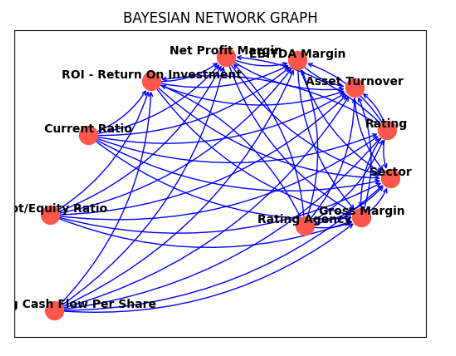
\includegraphics[scale=0.8]{img/bn.png}
\end{figure}
\noindent Di seguito si riporta l'esempio di una \textit{CPD}:

\begin{figure}[H]
    \centering
    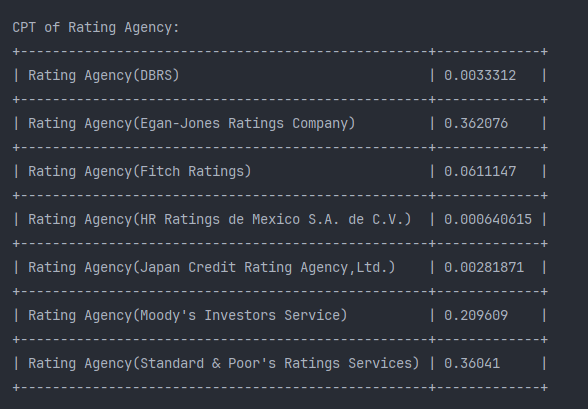
\includegraphics[scale=0.6]{img/cpt.png}
\end{figure}
\noindent Non si è riuscito ad ottenere in tempi ragionevoli la stampa della CPT di una variabile avente dei parents, dato che la rete è molto complessa.

\subsection{Generazione di sample e gestione di dati mancanti}
\noindent Tramite la rete bayesiana è possibile generare nuovi sample, ovvero nuove configurazioni di variabili. Questo è utile per generare nuovi dati da utilizzare per addestrare un modello, o per fare inferenza su nuovi dati.  
\\ Le reti bayesiane sono in grado di gestire casi in cui una variabile di input non è nota. Questo è utile in quanto i dati reali spesso presentano valori mancanti. La rete bayesiana è in grado di fare inferenza su nuovi dati, anche se non tutte le variabili sono note.

\begin{figure}[H]
    \centering
    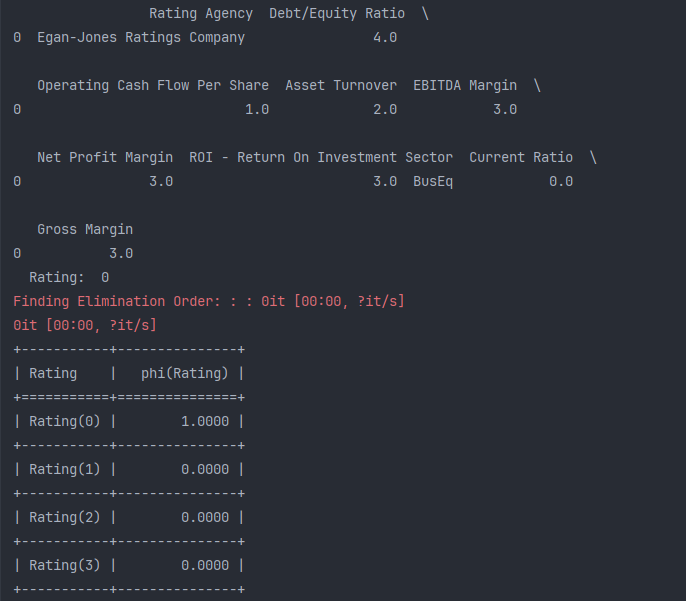
\includegraphics[scale=0.5]{img/sample_generated_bn.png}
    \caption{Esempio generato e classificato}
    \label{fig:normal}
\end{figure}

\begin{figure}[H]
    \centering
    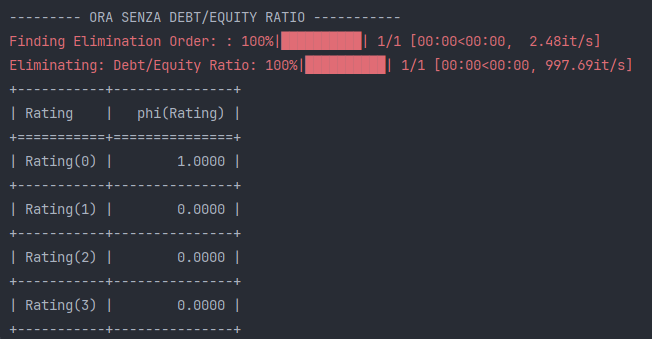
\includegraphics[scale=0.5]{img/sample_generated_bn_without.png}
    \caption{Esempio generato e classificato senza \textit{Debt/Equity Ratio}}
    \label{fig:without}
\end{figure}

\begin{figure}[H]
    \centering
    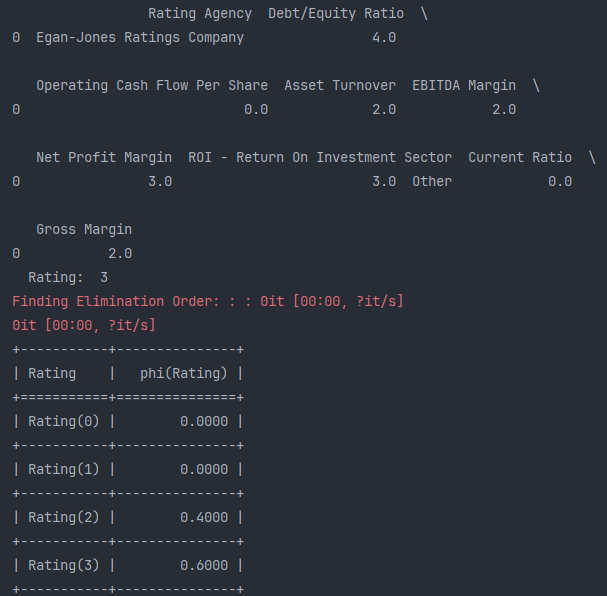
\includegraphics[scale=0.5]{img/so_so.png}
    \caption{Distribuzione di probabilità ampia}
    \label{fig:so}
\end{figure}
\begin{figure}[H]
    \centering
    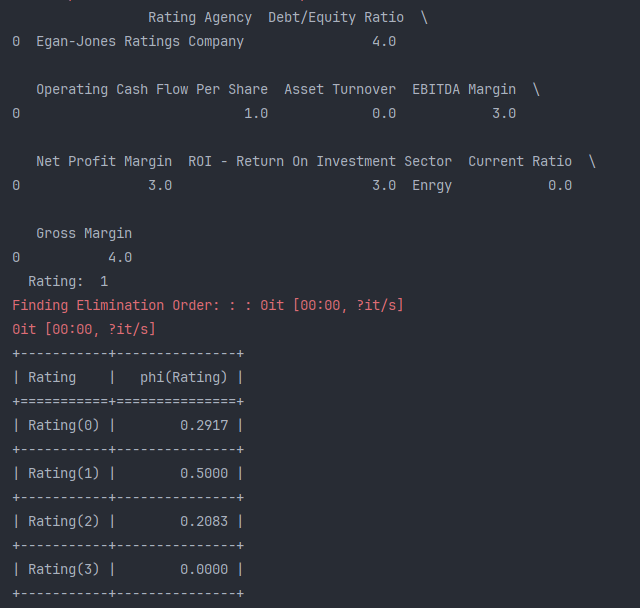
\includegraphics[scale=0.5]{img/bad_prob.png}
    \caption{Distribuzione di probabilità molto ampia}
    \label{fig:bad}
\end{figure}

\noindent Come è possibile notare la rete è in grado di fare inferenza sulla variabile \textit{Rating} anche se non sono note delle variabili, come nel nostro caso di \textit{Debt/Equity Ratio} in $Figura$ \ref{fig:without}.
\\ E' anche possibile notare che non sempre la rete riesce ad assegnare una stima esatta come in $Figura$ \ref{fig:bad}. Alcune volte riesce a stimare una probabilità vicina come in $Figura$ \ref{fig:so}, altre volte invece la distribuzione di probabilità è molto più ampia come in $Figura$ \ref{fig:bad}, riuscendo però comunque a fornire la probabilità più alta alla classe corretta.

\subsection{Valutazione}

\noindent E' possibile stabilire quanto bene il modello descrive i dati osservati. Questo è utile per valutare la bontà del modello. Utilizzeremo il \textit{correlation-score} offerto da \textit{pgmpy}, che effettua un test di correlazione tra le variabili del dataset.\\ Il correlation-score della nostra rete bayesiana rispetto alla sua \textit{balanced accuracy} è circa $0.59$, questo indica che la rete è in grado di catturare una certa correlazione tra le variabili, ma non è in grado di catturare tutte le dipendenze probabilistiche tra le variabili.

\subsection{Query di esempio}
\noindent Le reti bayesiane sono in grado di rispondere a query probabilistiche, ovvero di calcolare la probabilità di una variabile dato un insieme di evidenze. Di seguito si riportano due esempi di query:

\begin{figure}[H]
    \centering
    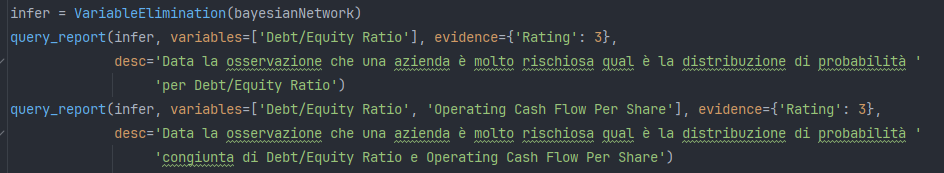
\includegraphics[scale=0.5]{img/ex_query.png}
    \caption{Esempio di query}
\end{figure}

\begin{itemize}[label=-]
    \item Data l'osservazione che una azienda è molto rischiosa qual è la distribuzione di probabilità per \textit{Debt/Equity Ratio}
    \item Data l'osservazione che una azienda è molto rischiosa qual è la distribuzione di probabilità congiunta di \textit{Debt/Equity Ratio} e \textit{Operating Cash Flow Per Share}
\end{itemize}

\begin{figure}[H]
    \centering
    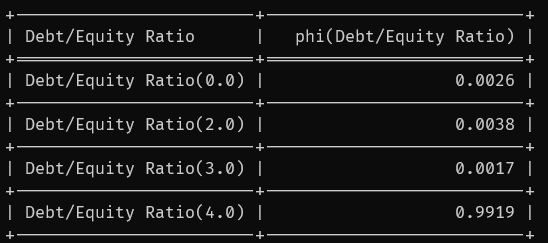
\includegraphics[scale=0.5]{img/firstq.png}
    \caption{Risultato prima query}
\end{figure}

\begin{figure}[H]
    \centering
    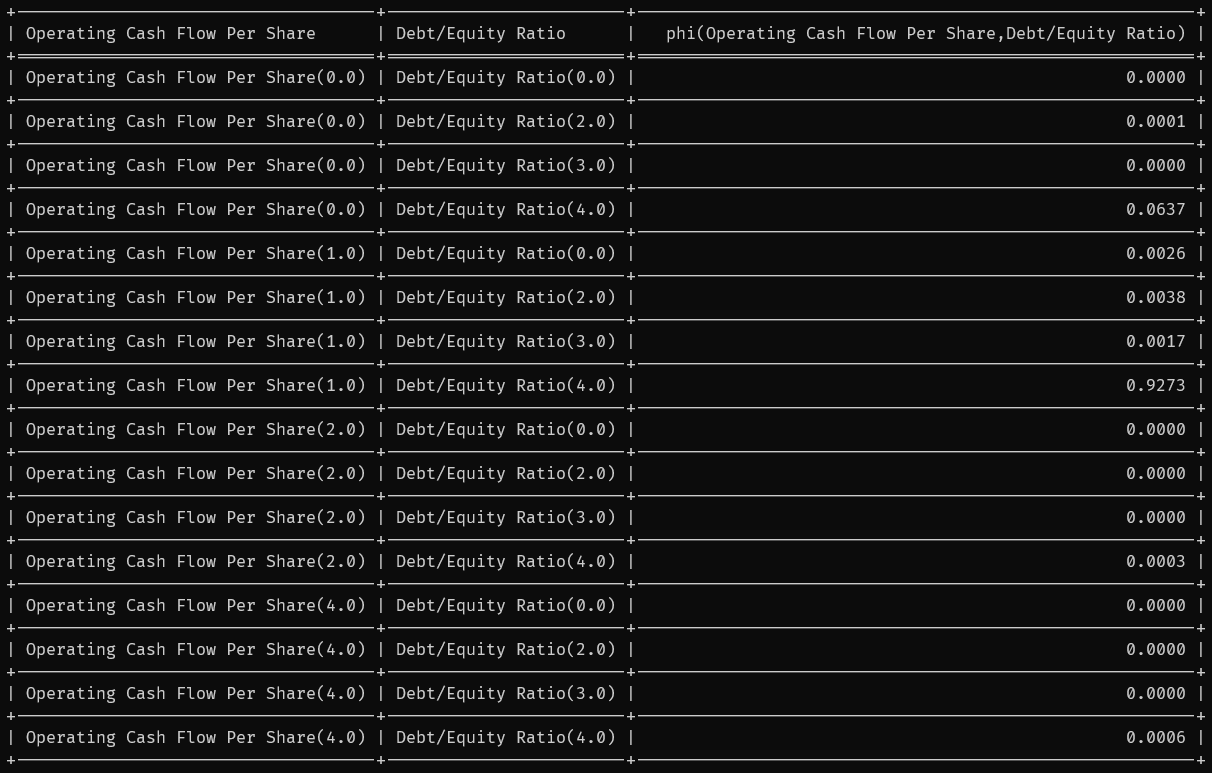
\includegraphics[scale=0.5]{img/secondq.png}
    \caption{Risultato seconda query}
\end{figure}

\noindent Da query di questo tipo possiamo ottenere informazioni utili per trarre delle conclusioni, ad esempio che un'azienda molto rischiosa ha molto probabilmente un \textit{Debt/Equity Ratio} alto, e che quindi tende ad indebitarsi. Dalla seconda query notiamo che se un'azienda è molto rischiosa allora questa ha molto probabilmente un \textit{Debt/Equity Ratio} alto e un \textit{Operating Cash Flow Per Share} basso.

\subsection{Sommario}

\noindent Dato lo sbilanciamento delle classi, e dato il numero minore di esempi su cui è stato allenata la rete bayesiana, dato che eliminando delle feature molti esempi risultavano duplicati, possiamo tutto sommato dire che la rete bayesiana creata ha delle prestazioni accettabili, e permette di eseguire delle query probabilistiche interessanti.